%%
%% This is file `hustreport-zh-example.tex',
%% generated with the docstrip utility.
%%
%% The original source files were:
%%
%% hustreport.dtx  (with options: `example-zh')
%% 
%% This is a generated file.
%% 
%% Copyright (C) 2013-2014 by Xu Cheng <xucheng@me.com>
%%               2014-2016 by hust-latex <https://github.com/hust-latex>
%% 
%% This work may be distributed and/or modified under the
%% conditions of the LaTeX Project Public License, either version 1.3
%% of this license or (at your option) any later version.
%% The latest version of this license is in
%%   http://www.latex-project.org/lppl.txt
%% and version 1.3 or later is part of all distributions of LaTeX
%% version 2005/12/01 or later.
%% 
%% This work has the LPPL maintenance status `maintained'.
%% 
%% The Current Maintainer of this work is hust-latex Organization.
%% 
%% This work consists of the files hustreport.dtx,
%% hustreport.ins and the derived file hustreport.cls
%% along with its document and example files.
%% 
%% \CharacterTable
%% {Upper-case    \A\B\C\D\E\F\G\H\I\J\K\L\M\N\O\P\Q\R\S\T\U\V\W\X\Y\Z
%%  Lower-case    \a\b\c\d\e\f\g\h\i\j\k\l\m\n\o\p\q\r\s\t\u\v\w\x\y\z
%%  Digits        \0\1\2\3\4\5\6\7\8\9
%%  Exclamation   \!     Double quote  \"     Hash (number) \#
%%  Dollar        \$     Percent       \%     Ampersand     \&
%%  Acute accent  \'     Left paren    \(     Right paren   \)
%%  Asterisk      \*     Plus          \+     Comma         \,
%%  Minus         \-     Point         \.     Solidus       \/
%%  Colon         \:     Semicolon     \;     Less than     \<
%%  Equals        \=     Greater than  \>     Question mark \?
%%  Commercial at \@     Left bracket  \[     Backslash     \\
%%  Right bracket \]     Circumflex    \^     Underscore    \_
%%  Grave accent  \`     Left brace    \{     Vertical bar  \|
%%  Right brace   \}     Tilde         \~}
\documentclass[format=draft,language=chinese,category=academic-report]{hustreport}

\stuno{1111}
\title{基于前馈神经网络的分类任务设计}
\author{thezmmm}
\major{数据科学与大数据技术}
\class{000}
\advisor{杨卫}

\begin{document}

\frontmatter
\maketitle
\tableofcontents
\mainmatter

\chapter{实验要求}
\begin{enumerate}
\item 实验目标:

设计一个前馈神经网络,将给定的二维高斯数据集进行分类。

\item 数据集描述:

下载并导入名为"dataset.csv"的数据集。该数据集包含四类二维高斯数据和它们的标签。数据集中的每个样本由两个特征值(〖data〗\_1, 〖data〗\_2)和对应的分类标签组成。

\item 数据预处理:

随机排序:首先对数据集进行随机排序,以确保训练集和测试集的样本分布均匀。
划分训练集和测试集:将排序后的数据集划分为训练集和测试集。其中90\%的数据将用于训练,剩下的10\%用于测试。
\item 神经网络设计:

前馈神经网络:设计一个前馈神经网络,用于分类任务。
隐藏层:至少包含一层隐藏层,可以根据需要选择隐藏层的数量和神经元的数量。
输入层:输入层的节点数量应与数据集中的特征数量相匹配,即两个。
输出层:输出层的节点数量应与分类任务的类别数量相匹配,即四个。
\item 训练和测试:

使用划分好的训练集对神经网络进行训练。
使用划分好的测试集对神经网络进行测试和评估。
可以选择适当的训练算法和评估指标,如反向传播算法和准确率。
\item 实验结果:

给出实验结果的详细记录,包括训练过程中的损失值变化和测试集上的准确率等。
可以使用图表、表格或其他形式展示实验结果。 
\end{enumerate}
\chapter{实验内容}
\section{数据集划分}
数据集的准备过程如下:
\begin{enumerate}
\item 加载数据集:

使用`pd.read\_csv()`函数加载名为"dataset.csv"的数据集文件,并将其存储在一个名为`data`的变量中。

\item 随机排序数据集:

使用`sample()`函数和`frac`参数设置为1,对数据集进行随机排序。`frac=1`表示保留全部数据,实现了对整个数据集的洗牌操作。通过`reset\_index(drop=True)`将重置索引,确保数据集的索引是连续的。

\item 提取特征和标签:

从排序后的数据集中提取特征和标签。将`data`中名为'data1'和'data2'的列提取出来,使用`values`属性将其转换为NumPy数组,并将其存储在一个名为`features`的变量中。同时,将`data`中名为'label'的列提取出来,使用`values`属性将其转换为NumPy数组,并将其存储在一个名为`labels`的变量中。这样,`features`变量将包含二维高斯数据的特征,而`labels`变量将包含对应的分类标签。

\item 划分训练集和测试集:

使用`train\_test\_split()`函数将数据集划分为训练集和测试集。将`features`和`labels`作为输入参数,通过`test\_size`参数设置测试集的比例,这里设置为0.1表示测试集占总样本数的10\%。通过`random\_state`参数设置随机种子,以确保划分结果的可重复性。将划分后的训练集特征、测试集特征、训练集标签和测试集标签分别存储在`train\_features`、`test\_features`、`train\_labels`和`test\_labels`变量中。
\end{enumerate}
\begin{lstlisting}
# 加载数据集
data = pd.read_csv('dataset.csv')

# 随机排序数据集
data = data.sample(frac=1).reset_index(drop=True)

# 提取特征和标签
features = data[['data1', 'data2']].values
labels = data['label'].values - 1

# 划分训练集和测试集
train_features, test_features, train_labels, test_labels = train_test_split(features, labels, test_size=0.1, random_state=42)
\end{lstlisting}
\section{神经网络模型}
\begin{lstlisting}
# 定义神经网络的架构
model = tf.keras.Sequential([
    tf.keras.layers.Dense(64, activation=activation_function, input_shape=(2,)),
    tf.keras.layers.Dense(32, activation=activation_function),
    tf.keras.layers.Dense(4, activation='softmax')
])
\end{lstlisting}
这段代码定义了神经网络的架构,它是一个序列模型(Sequential Model)。

\begin{enumerate}
\item 第一层是一个全连接层(Dense Layer),它有64个神经元。这一层使用了一个激活函数(activation\_function),实验中使用了ReLU和sigmoid两种激活函数。激活函数的作用是引入非线性性质,以便网络可以学习复杂的模式和关系。这一层的输入形状为(2,),表示输入数据的维度是2。

\item 第二层也是一个全连接层,有32个神经元,并且也使用了相同的激活函数。这一层没有指定输入形状,因为它会自动适应前一层的输出形状作为输入。

\item 最后一层是一个全连接层,有4个神经元,并使用了softmax激活函数。softmax函数将神经元的输出转化为概率分布,用于多分类问题。这一层的输出表示模型对输入数据属于每个类别的概率分布。

\end{enumerate}
这个神经网络的输入层有2个特征,输出层有4个类别。中间的两个全连接层为网络提供了学习和表示数据的能力。整个网络的结构是一个前馈神经网络,每一层的输出作为下一层的输入,信息从前向后传播。实验中根据具体的需求,调整了网络的层数、每层的神经元数量以及激活函数等参数,从而获得不同的实验结果以供分析。

\begin{figure}[htbp]
\centering
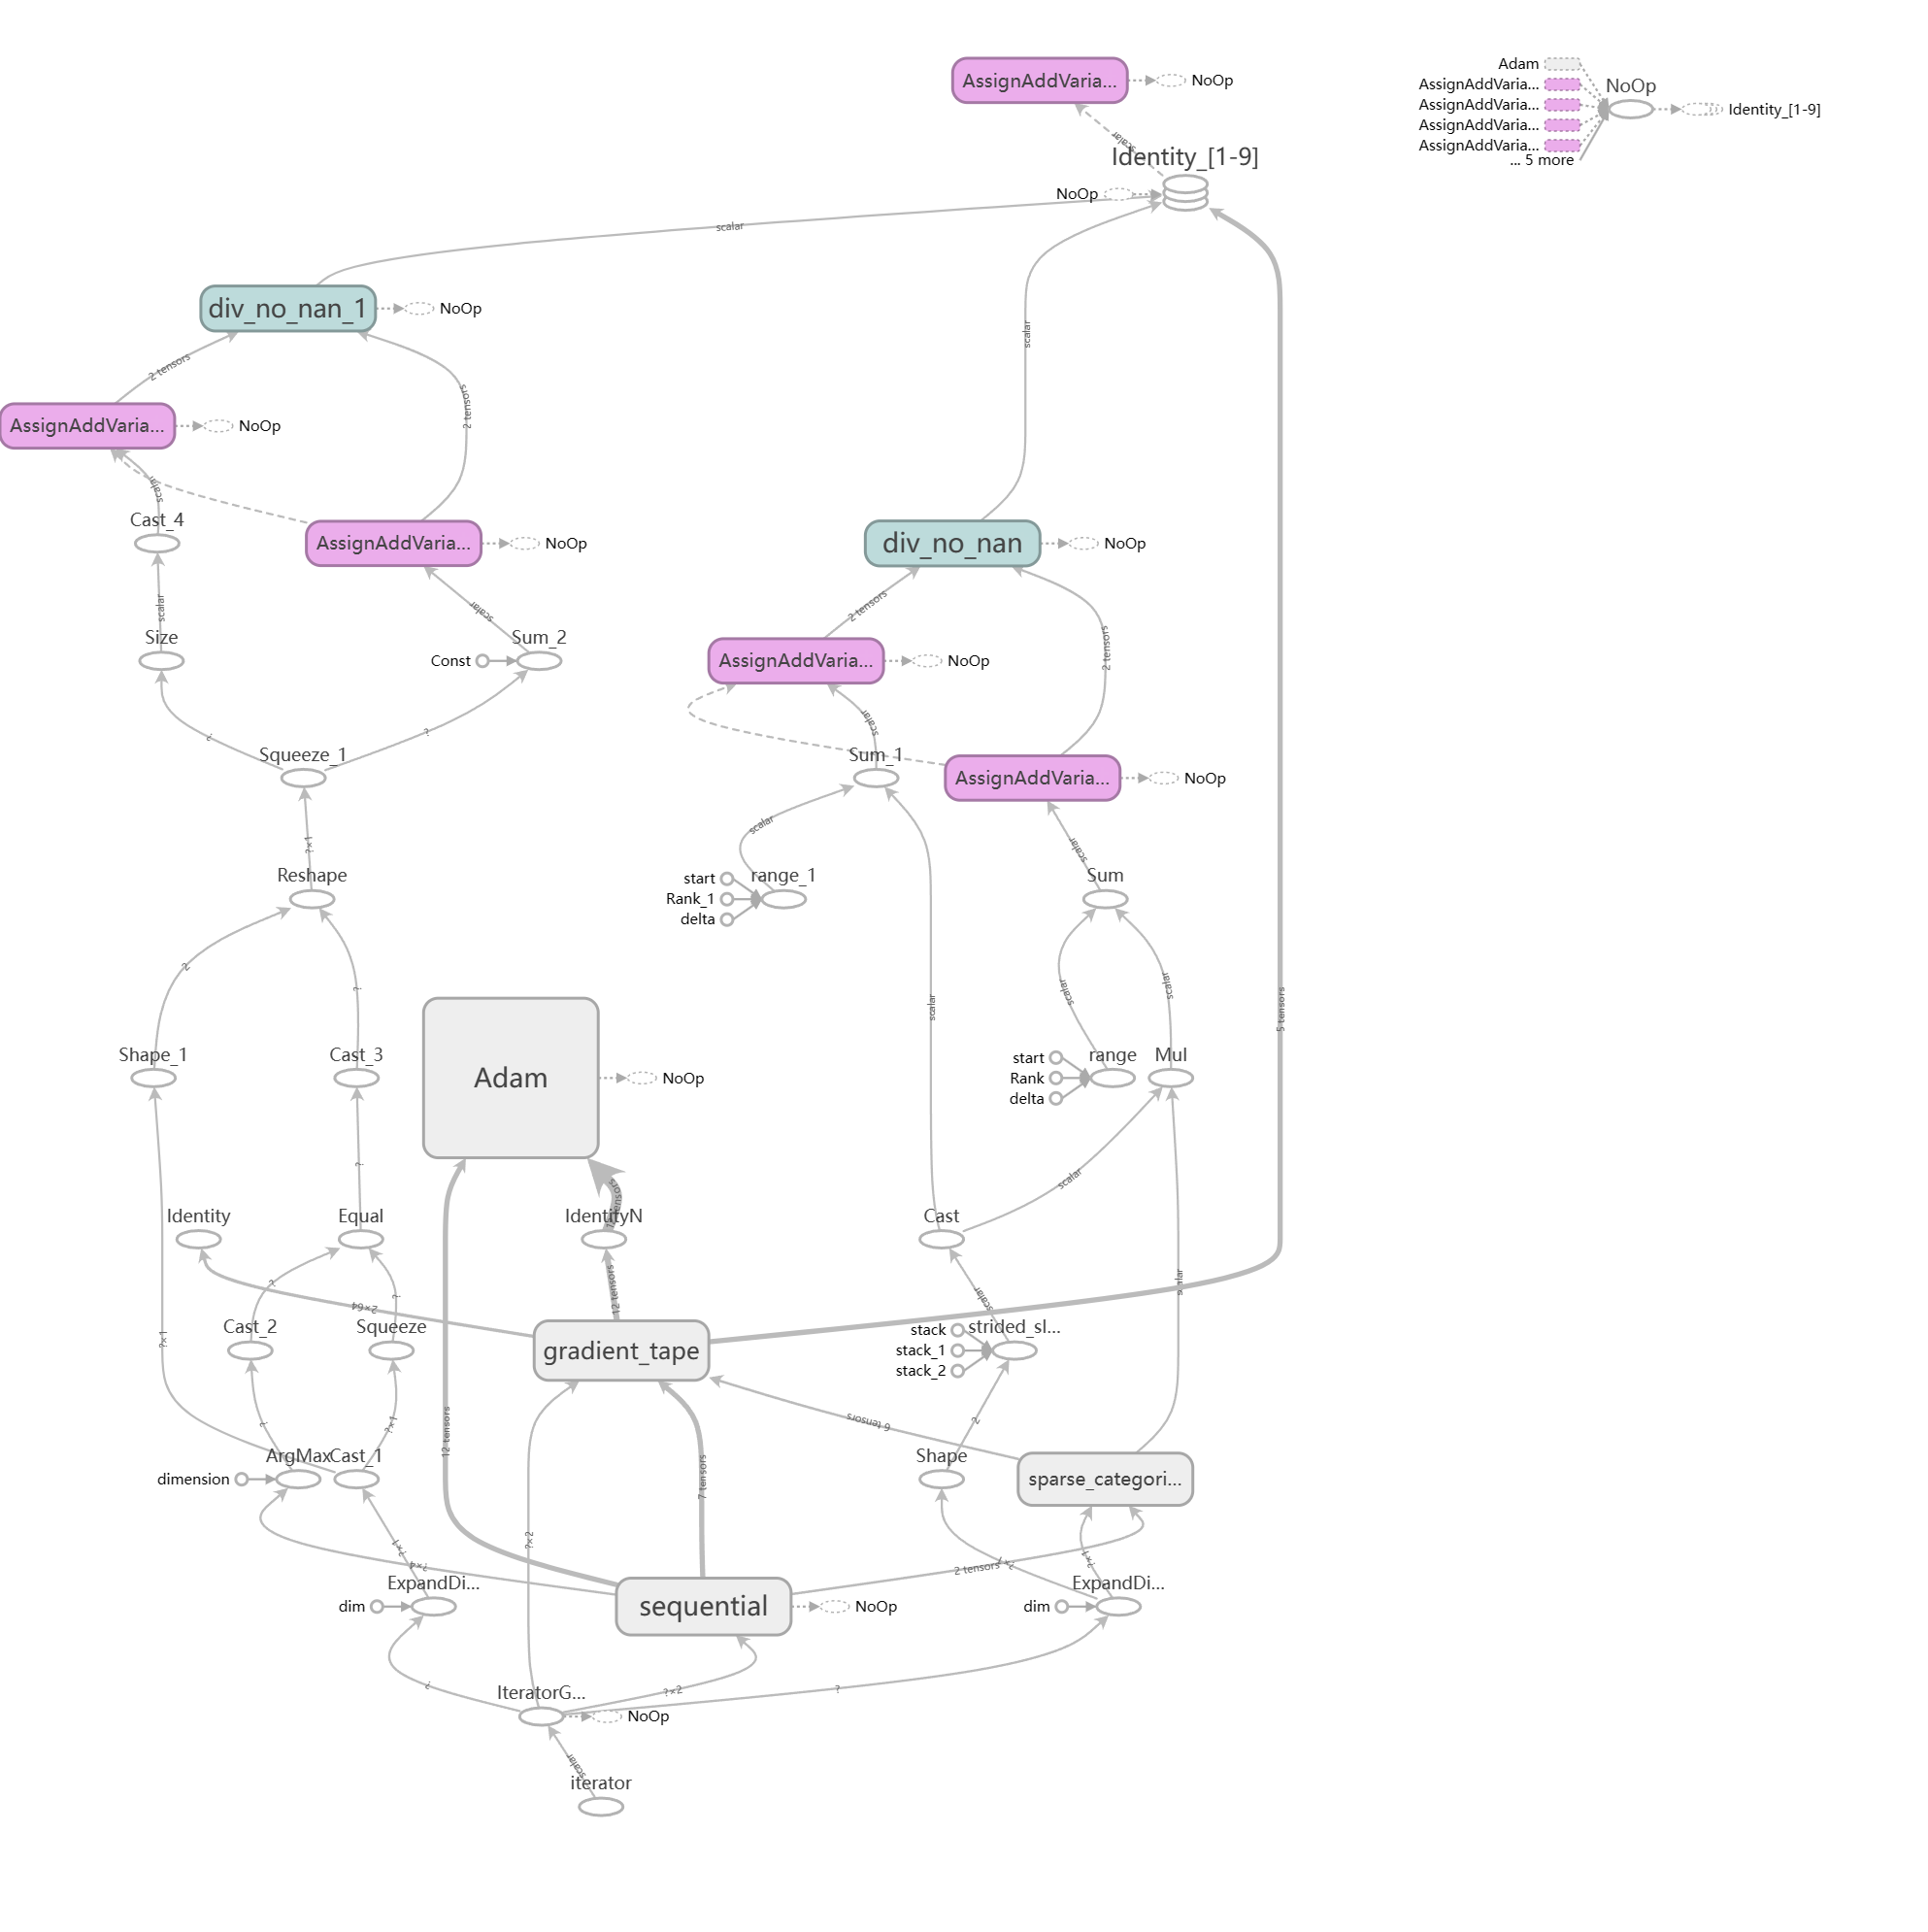
\includegraphics[scale=0.3]{img/layers_3_neurons_100_activation_relu_train.png}
\caption{神经网络架构图}
\end{figure}

\section{网络参数}
\subsection{网络层数}
指定神经网络的层数,即网络中包含的全连接层的数量。在给定的代码中,神经网络有3层,包括输入层、一个隐藏层和输出层。实验过程中尝试了两层神经网络。
\subsection{神经元数量}
指定每个全连接层中的神经元数量之和。其中,每一层的神经元数量都为$2^n$。
\subsection{激活函数}
激活函数是应用于每个神经元的非线性函数。在实验过程中,使用了三种激活函数:ReLU(修正线性单元),Sigmoid和tanh。ReLU对于隐藏层常用,它将负输入值设置为零,并保持正输入值不变。Sigmoid函数则将输入值映射到0到1之间的连续值,常用于二分类问题或输出层的概率估计。tanh函数的图像与sigmoid十分相似,它的输出取值是(-1, 1),也具有同样的缺点,梯度消失,计算复杂。
\subsection{优化器}
优化器决定了神经网络在训练过程中如何更新权重以最小化损失函数。在实验过程中,使用了Adam优化器,它是一种基于梯度的优化算法,结合了动量方法和自适应学习率。
\subsection{损失函数}
损失函数用于衡量模型预测与实际标签之间的差异。在实验过程中,使用了稀疏分类交叉熵损失函数(sparse\_categorical\_crossentropy),适用于多分类问题,并且标签是整数形式。
\subsection{训练轮数}
指定神经网络在训练数据上迭代的次数。在实验过程中,网络将在训练数据上进行10个轮次的迭代。
\subsection{批量大小}
指定每个训练批次中使用的样本数量。在实验过程中,每个批次包含32个样本。
\chapter{实验结果}
\section{迭代次数的影响}
根据提供的实验结果,可以分析迭代次数(Epochs)对网络性能的影响。
\begin{figure}[htbp]
\centering
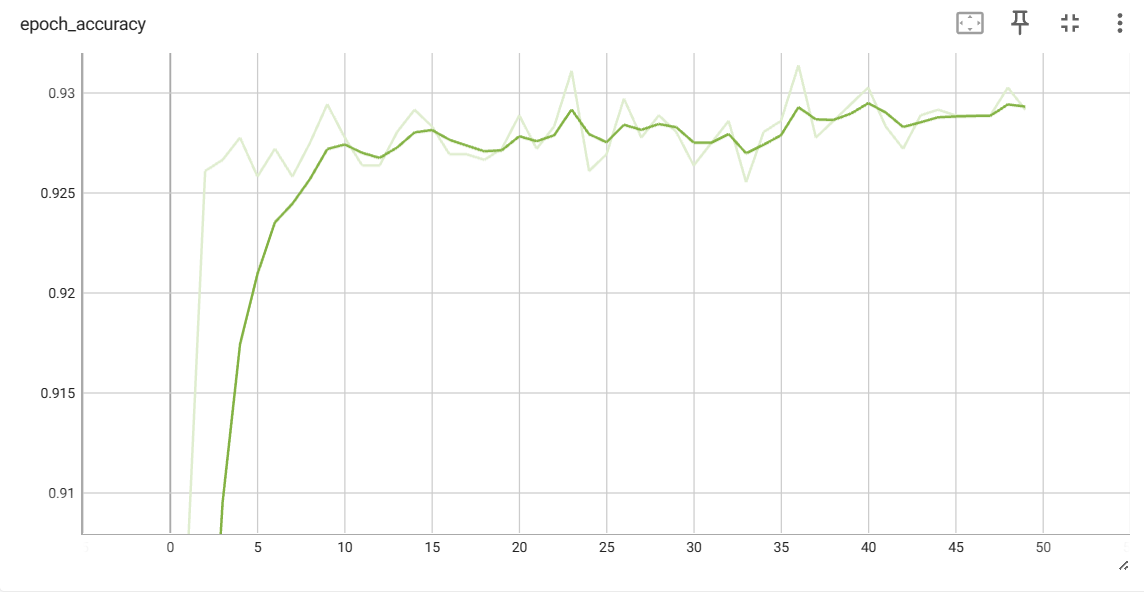
\includegraphics[scale=0.4]{img/epoch_accuracy_epoch.png}
\caption{epoch\_accuracy}
\end{figure}
\begin{figure}[htbp]
\centering
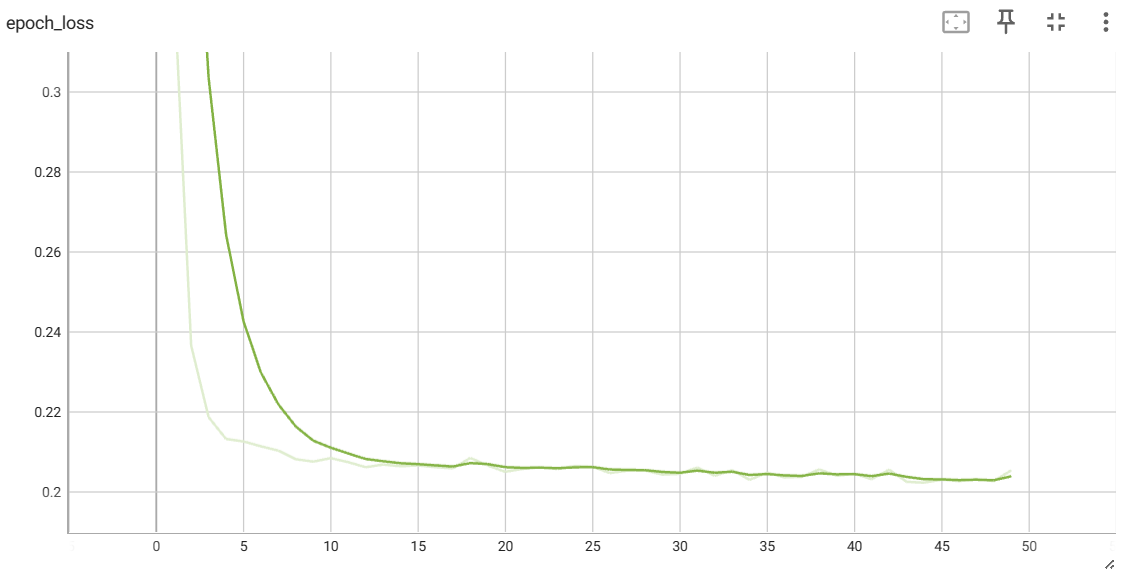
\includegraphics[scale=0.4]{img/epoch_loss_epoch.png}
\caption{epoch\_loss}
\end{figure}
\begin{enumerate}
\item 迭代次数对准确度的影响:
\begin{itemize}
\item 随着迭代次数的增加,准确度逐渐提高,从初始的0.788888872逐渐增加到最高的0.931388915。
\item 在迭代次数较低时,准确度的提升较为明显,但随着迭代次数的增加,提升幅度逐渐减小。
\item 在最后几次迭代中,准确度相对稳定,没有明显的进一步改善。
\end{itemize}
\item 迭代次数对损失函数的影响:
\begin{itemize}
\item 随着迭代次数的增加,损失函数的值逐渐减小,从初始的0.83936125逐渐降低到最低的0.202553749。
\item 在迭代次数较低时,损失函数的下降较为明显,但随着迭代次数的增加,下降速度逐渐变慢。
\item 在最后几次迭代中,损失函数的值相对稳定,没有明显的进一步改善。
\end{itemize}
\end{enumerate}
根据实验结果,随着迭代次数的增加,模型的性能有所改善,准确度提高,损失函数降低。

在较低的迭代次数时,模型可能还没有充分学习数据集的特征和模式,因此准确度较低,损失函数较高。

随着迭代次数的增加,模型逐渐学习到更多的特征和模式,准确度提高,损失函数降低。

在一定程度上,模型的性能可能会随着迭代次数的增加而趋于稳定,准确度和损失函数的改善幅度减小。
\section{激活函数的影响}
根据实验结果,可以对三种不同的激活函数(ReLU、Sigmoid和Tanh)对网络性能的影响进行分析。下面是对每个激活函数的影响进行详细分析:
\begin{figure}[htbp]
\centering
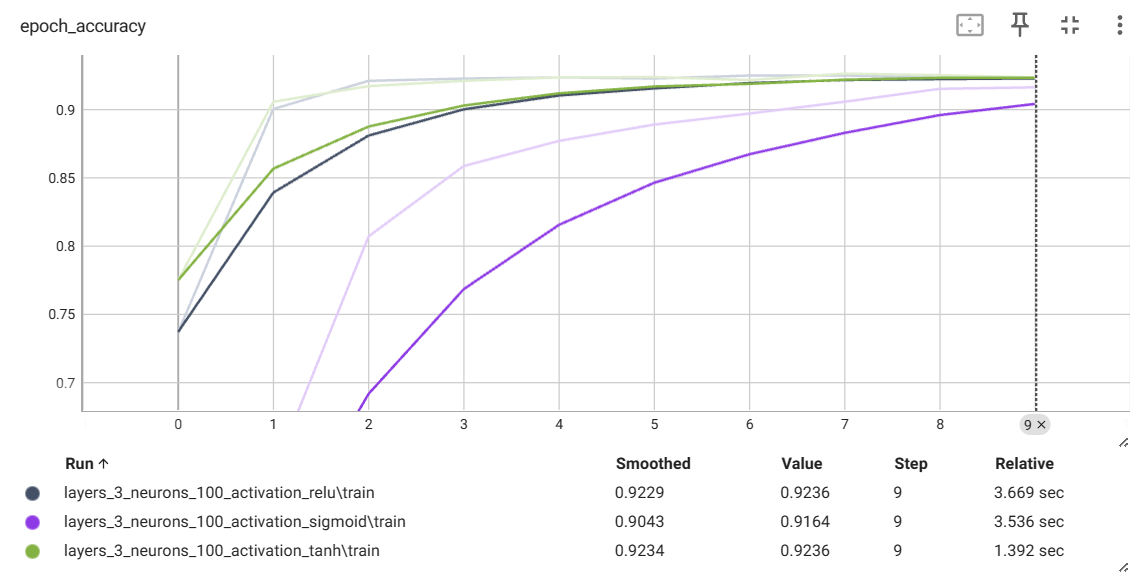
\includegraphics[scale=0.4]{img/epoch_accuracy_activation.png}
\caption{不同激活函数的准确度}
\end{figure}
\begin{figure}[htbp]
\centering
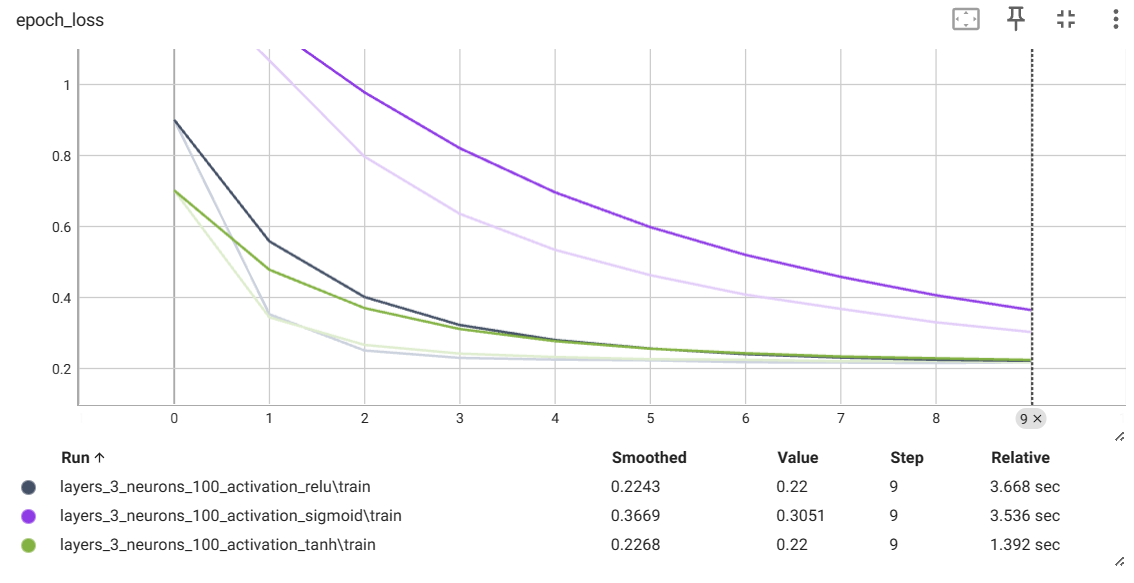
\includegraphics[scale=0.4]{img/epoch_loss_activation.png}
\caption{不同激活函数的损失值}
\end{figure}
\begin{enumerate}
\item ReLU激活函数:

准确率:在10个训练轮次中,准确率从初始值0.738逐渐增加到0.924,显示出较好的收敛性。然而,准确率在后续的轮次中没有明显的提升,可能暗示网络已经接近其性能上限。

损失值:损失值从初始值0.901下降到0.220,在每个轮次中都有显著的减少。这表明模型在训练过程中有效地减小了预测值与实际标签之间的差距。
\item Sigmoid激活函数:

准确率:在10个训练轮次中,准确率从初始值0.469逐渐增加到0.916。相对于ReLU函数,Sigmoid函数的准确率增长速度较慢,并且在后续轮次中的增长也相对较小。

损失值:损失值从初始值1.330下降到0.305,在每个轮次中都有显著的减少。然而,相对于ReLU函数,Sigmoid函数的损失值要高得多。
\item Tanh激活函数:

准确率:在10个训练轮次中,准确率从初始值0.776逐渐增加到0.924。Tanh函数的准确率增长速度与ReLU函数相当,但整体性能略低于ReLU函数。

损失值:损失值从初始值0.703下降到0.220,在每个轮次中都有显著的减少。Tanh函数的损失值与ReLU函数相当。
\end{enumerate}

在这个特定的实验设置中,ReLU激活函数表现出最佳的性能,具有较高的准确率和较低的损失值。这可能是因为ReLU函数能够更好地处理梯度消失问题,并在训练过程中提供更好的非线性拟合能力。

Sigmoid激活函数在准确率和损失值方面的表现相对较差,可能是因为其饱和性导致了梯度消失问题,并且在深层网络中较难优化。

Tanh激活函数的性能介于ReLU和Sigmoid之间,虽然能够处理梯度消失问题,但相对于ReLU函数,它的性能略低。

总的来说,激活函数对神经网络的性能有明显的影响。在实验结果中,ReLU激活函数在这个特定的任务上表现最好,但对于不同的数据集和任务,不同的激活函数可能会有不同的效果。因此,在选择激活函数时,需要根据具体情况和实验结果进行评估和选择。
\section{网络层数及神经元数量的影响}
\begin{figure}[htbp]
\centering
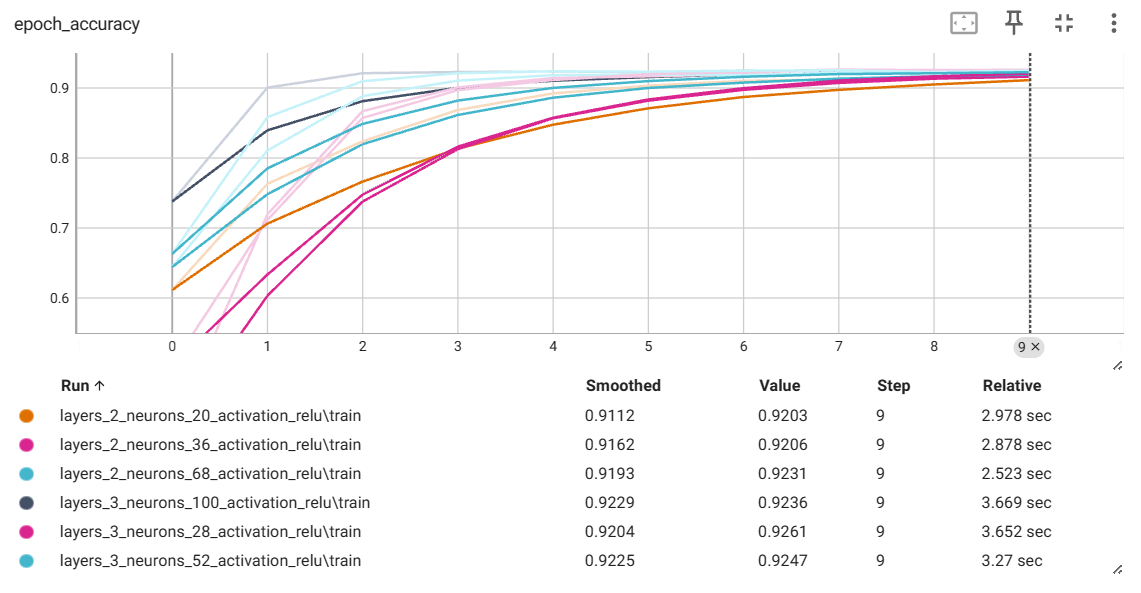
\includegraphics[scale=0.4]{img/epoch_accuracy_num.png}
\caption{不同网络层数和神经元数量的准确度}
\end{figure}
\begin{figure}[htbp]
\centering
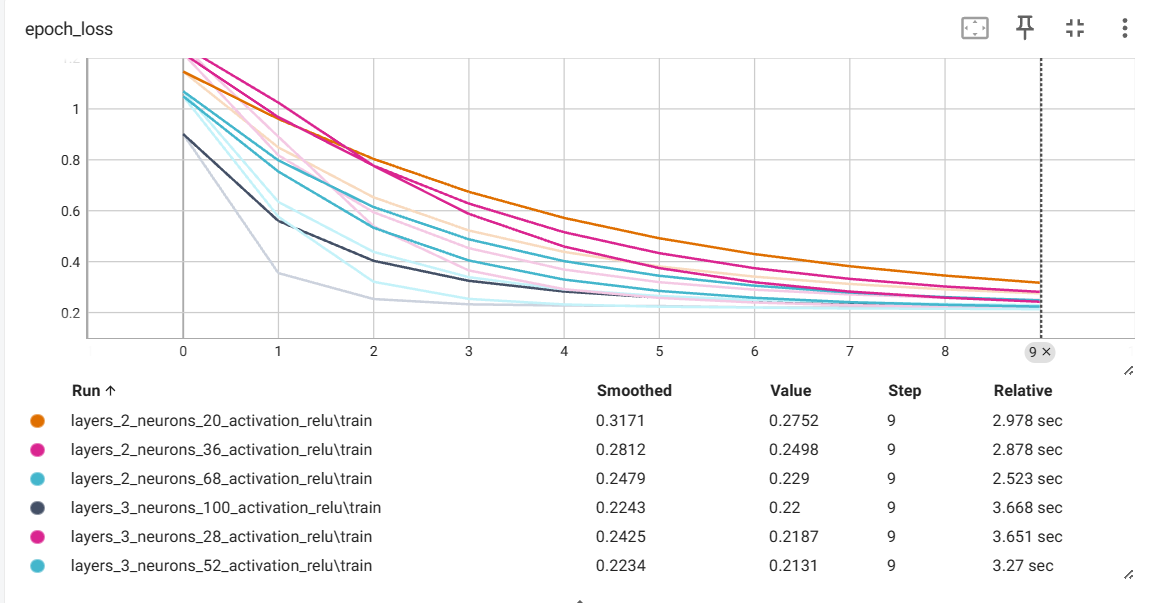
\includegraphics[scale=0.4]{img/epoch_loss_num.png}
\caption{不同网络层数和神经元数量的损失值}
\end{figure}
\subsection{神经元数量的影响}
在2层网络中,增加神经元数量从20到36时,准确性(accuracy)有所提高,从0.920277774增加到0.920555532。然而,当神经元数量增加到68时,准确性提高到0.92305553,比36神经元更高。这表明增加神经元数量可以改善网络性能,但超过一定点后,进一步增加神经元数量可能带来较小的性能改善。

在3层网络中,增加神经元数量从28到52时,准确性从0.926111102提高到0.924722195。然而,当神经元数量增加到100时,准确性下降到0.219961464,比52神经元更低。这表明增加神经元数量可以提高性能,但超过一定点后,可能会导致过拟合和性能下降。
\subsection{网络层数的影响}
在2层网络中,网络的准确性逐渐提高,从0.920277774到0.92305553,随着神经元数量的增加。这说明在一定范围内,增加网络层数可以提高性能。

在3层网络中,准确性从0.926111102到0.924722195,随着神经元数量的增加而略微下降。这表明增加网络层数不一定会带来更好的性能,而是取决于其他因素,如神经元数量和数据集的复杂性。
\subsection{总结}
综合考虑神经元数量和网络层数的影响,我们可以得出以下结论:
\begin{enumerate}
\item 增加神经元数量可以提高网络性能,但超过一定点后,进一步增加可能带来较小的改进或导致性能下降。
\item 增加网络层数可以在一定范围内提高性能,但过多的层数不一定会带来更好的结果。
\item 在确定最佳神经元数量和网络层数时,需要综合考虑模型的准确性、过拟合风险和计算资源的限制。
\end{enumerate}

\chapter{总结}
本次实验设计了基于前馈神经网络的四分类神经网络模型,分析了神经网络性能受到的多个因素的影响,包括迭代次数、激活函数、网络层数、神经元数量。以下是对这些因素的概括性总结:
\begin{enumerate}
\item 迭代次数:增加迭代次数可以改善神经网络性能,提高准确度并降低损失函数。然而,性能的改善幅度会逐渐减小,需要在时间和性能改善之间进行权衡。

\item 激活函数:激活函数的选择对网络性能至关重要。常见的激活函数有ReLU、Sigmoid、Tanh和Leaky ReLU等,具体选择要根据任务和数据特性进行调整。

\item 网络层数:增加网络层数可以增强网络的表达能力,但同时也增加了过拟合的风险。适当的网络层数取决于任务的复杂性和可用的训练数据量。

\item 神经元数量:适当的神经元数量可以提高网络的表达能力,但过多的神经元可能导致过拟合。选择合适的神经元数量需要在模型复杂性和计算资源之间进行平衡。
\end{enumerate}
综上所述,选择适当的迭代次数、激活函数、网络层数、神经元数量和模型架构是优化神经网络性能的关键因素,需要综合考虑任务要求和数据特性来进行调整和优化。
\end{document}
\endinput
%%
%% End of file `hustreport-zh-example.tex'.
